\documentclass[10pt,pdf,hyperref={unicode}]{beamer}

\mode<presentation>
{
\usetheme{boxes}
\beamertemplatenavigationsymbolsempty

\setbeamertemplate{footline}[page number]
\setbeamersize{text margin left=0.5em, text margin right=0.5em}
}

\usepackage[utf8]{inputenc}
\usepackage[english, russian]{babel}
\usepackage{bm}
\usepackage{multirow}
\usepackage{ragged2e}
\usepackage{indentfirst}
\usepackage{multicol}
\usepackage{subfig}
\usepackage{amsmath,amssymb}
\usepackage{enumerate}
\usepackage{mathtools}
\usepackage{comment}
\usepackage{multicol}

\usepackage[all]{xy}

\usepackage{tikz}
\usetikzlibrary{positioning,arrows}

\tikzstyle{name} = [parameters]
\definecolor{name}{rgb}{0.5,0.5,0.5}

\usepackage{caption}
\captionsetup{skip=0pt,belowskip=0pt}

\newtheorem{rustheorem}{Теорема}
\newtheorem{russtatement}{Утверждение}
\newtheorem{rusdefinition}{Определение}

% colors
\definecolor{darkgreen}{rgb}{0.0, 0.2, 0.13}
\definecolor{darkcyan}{rgb}{0.0, 0.55, 0.55}

\AtBeginEnvironment{figure}{\setcounter{subfigure}{0}}

\captionsetup[subfloat]{labelformat=empty}

%----------------------------------------------------------------------------------------------------------

\title[]{Analysis of generative modeling methods based on Schrödinger bridges}
\author{Ksenofontov\,G.\,S.\\[1ex] 
\small Isachenko\,R.\,V.}
\institute[]{Moscow Institute of Physics and Technology}
\date[2023]{\small 20\;may\;2023}

%---------------------------------------------------------------------------------------------------------
\begin{document}

\begin{frame}
\titlepage
\end{frame}

%----------------------------------------------------------------------------------------------------------
\section{Research}
\begin{frame}{Research}
\bigskip
The problem of generating pictures using  Schrödinger bridge problem is investigated.
\begin{block}{Research objective~---}
suggest a method of improving diffusion models using Schrödinger bridges.
\end{block}
\begin{block}{Required to suggest}
\justifying
\begin{enumerate}[1.]
    \item theory to connect generative problem with Schrödinger bridge problem,
    \item method of fitting model using Schrödinger bridges.
\end{enumerate}
\end{block}
% \begin{block}{Solution}
% Для \ldots.
% \end{block}
\end{frame}
% %---------------------------------------------------------------------------------------------------------
\section{Problem statement}
\begin{frame}{Problem statement}
It is given
\begin{enumerate}[1.]
    \item $\{x_i\}_{i=0}^N \in \mathbb{R}^d$ -- dataset,
    \item $p_{prior}= \mathcal{N}(0, \textbf{I})$,
    \item $d\textbf{X}_t = f(t, \textbf{X}_t)dt + g(t)d\textbf{W}_t, X_0 \sim p_{data}$ -- forward process,
\end{enumerate}


\bigskip
We want to find reverse process, that goes from $p_{prior}$ to $p_{data}$. It solves using diffusion models minimizing sophisticated loss
$$d\textbf{X}t = [f(t, \textbf{X}_t) - g^2(t) s(t, \textbf{X}_t; \theta)]dt + g(t)d\textbf{W}_t, X_T \sim p_{prior},$$
where $t \in [0, T]$
However, when we solve this problem, we do not enforce the constraint on $X_T \sim p_{prior}$, thus it is practical task to find a good $T$ to get good approximation of $p_{prior}$

\end{frame}

% %----------------------------------------------------------------------------------------------------------
\section{Suggested Method}
\begin{frame}{Suggested Method}
~\\[-1mm]
Instead of considering the time-reversal of a forward noising process, let's build bridges (solve Schrödinger bridge problem) between the two boundary distributions and learn a mimicking diffusion process.
It is given
\begin{enumerate}[1.]
    \item $\mathbb{Q} \in \mathcal{P}(p_{data}, p_{prior})$ -- path measure of desired process,
    \item $\mathbb{P}$ -- path measure of forward process
\end{enumerate}

$$\min_{\mathbb{Q} \in \mathcal{P}(p_{data}, p_{prior})}D_{KL}(\mathbb{Q}||\mathbb{P})$$
The solution to the optimization can be expressed by the path measure of the following
forward, or equivalently backward, SDE
$$d\textbf{X}_t = [f(t, \textbf{X}_t) + g^2(t) \nabla_x\log\Psi(t, \textbf{X}_t)]dt+ g(t)d\textbf{W}_t, \textbf{X}_0 \sim p_{data}$$
$$d\textbf{X}_t = [f(t, \textbf{X}_t) - g^2(t) \nabla_x\log\hat\Psi(t, \textbf{X}_t)]dt+ g(t)d\textbf{W}_t, \textbf{X}_T \sim p_{prior}$$
$\Psi(t, \textbf{X}_t)$ and $\hat\Psi(t, \textbf{X}_t)$ are solution of duality problem of SBP
\end{frame}
%---------------------------------------------------------------------------------------------------------
\section{Related papers}
\begin{frame}{Related papers}
\begin{enumerate}[1.]
    \item \textit{Likelihood Training of Schrödinger Bridge using Forward-Backward SDEs Theory}\footnote{\url{https://arxiv.org/pdf/2110.11291.pdf}}: solving SB using duality problem
    \item \textit{Diffusion Schrödinger Bridge with Applications to Score-Based Generative Modeling}\footnote{\url{https://arxiv.org/pdf/2106.01357.pdf}}: solving SB using IPF algorithm on Dynamic Schrödinger Bridge problem
    \item \textit{Diffusion Schrödinger Bridge Matching}\footnote{\url{https://arxiv.org/pdf/2303.16852.pdf}}: solving SB using proposed algorithm IMF on Dynamic Schrödinger Bridge problem
\end{enumerate}
\end{frame}


%---------------------------------------------------------------------------------------------------------
\section{Future work plan}
\begin{frame}{Future work plan}
\begin{enumerate}[1.]
    \item Make a theory to connect SB and diffusion models
    \item Investigate $D_{KL}$ minimization, generalize to $f$-divergence.
\end{enumerate}
\end{frame}

% %----------------------------------------------------------------------------------------------------------
% \section{Анализ предложенного метода \ldots}
% \begin{frame}{Анализ предложенного метода \ldots}
% \justifying

% На графике показана зависимость значения параметров$w_i$ в зависимости от параметра~$l_1$-регуляризации~$C$.
% \begin{figure}[h!]
% 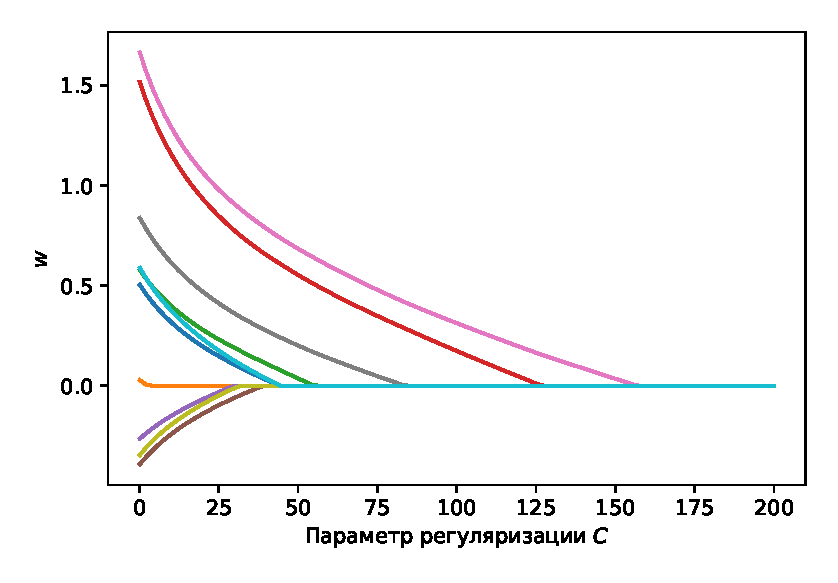
\includegraphics[width=0.45\textwidth]{../figures/log_reg_cs_exp.eps}
% 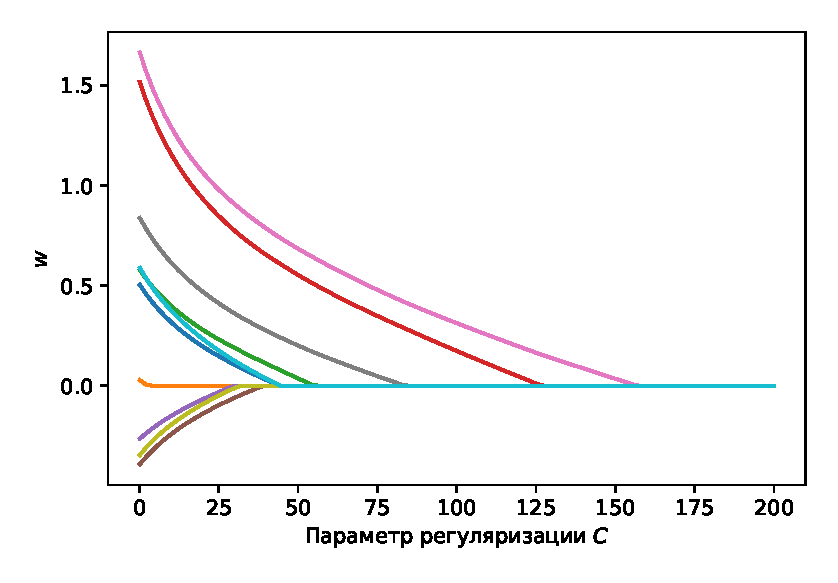
\includegraphics[width=0.45\textwidth]{../figures/log_reg_cs_exp.eps}
% \end{figure}

% С увеличением параметра регуляризации~$C$ число ненулевых параметров~$w_i$ уменьшается.

% \end{frame}

% %----------------------------------------------------------------------------------------------------------
% \section{Выводы}
% \begin{frame}{Выводы}
% \justifying
% 	\begin{enumerate}
% 	\justifying
% 	    \item Предложен \ldots.
%         \item Доказаны теоремы \ldots, 
%         \begin{itemize}
%             \item[---] \ldots,
%             \item[---] \ldots.
%         \end{itemize}
%         \item Предложен метод \ldots
%         \begin{itemize}
%             \item[---] \ldots,
%             \item[---] \ldots.
%         \end{itemize}
%         \item Предложены методы \ldots
%         \begin{itemize}
%             \item[---] \ldots,
%             \item[---] \ldots.
%         \end{itemize}
%         \item Предложена вероятностная интерпретации \ldots.
% 	\end{enumerate}
% \end{frame}
% %----------------------------------------------------------------------------------------------------------

\end{document} 